\section{Time plan (Gantt chart)}
\label{sect:timeplan}
As specified in section 7, the project consists of three basic work packages (each of them having several sub-packages):
\begin{itemize}
\item WP 1 - Basic research
\item WP 2 - Hardware and software development
\item WP 3 - Prototype development
\end{itemize}

\begin{figure}[H]
	\centering
    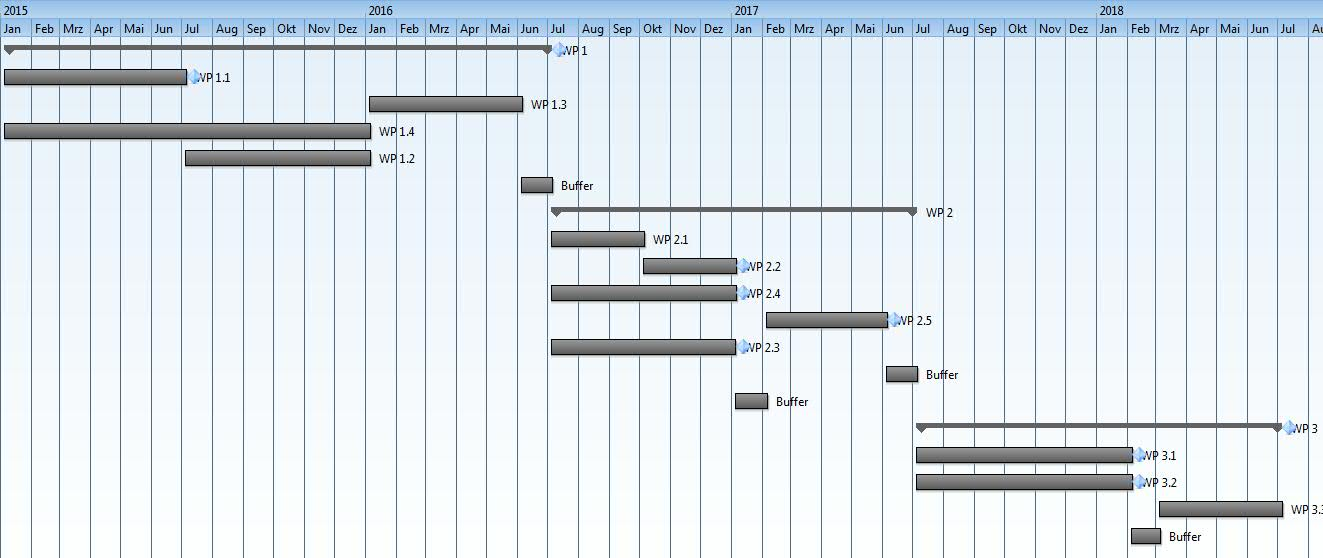
\includegraphics[width=1\textwidth]{gantt_chart}
    \caption{GANTT Chart}
\end{figure}

Each of these packages consists of another sub-packages. Since the research part of the project delivers the basis for the whole project and therefore is the most important part of the project, it has a planned duration of 1,5 years. The planned duration of the hardware and software development package is 1 year and the duration of the prototype development package 1 year. Also there is a scheduled time buffer of one month in each package, which can be used in potential problematic situations and in cases of time delays appearances. 

\subsection{Milestones}
The planned milestones of the projects are:
\begin{itemize}
\item 05.07.2015 - Confirmed uniqueness of a person’s brain wave pattern
\item 05.07.2016 - Research part completed 
\item 05.01.2017 - Hardware and Software for Microcontroller finished
\item 05.06.2017 - Hardware Part Completed 
\item 05.02.2018 - Prototype Completed 
\item 05.07.2018 - Project Completed 
\end{itemize}

\subsection{Timeplan}
The estimation of the schedule based on work packages:

\subsubsection{WP1 - Basic research}
\begin{itemize}
\item start date: 05.01.2015
\item end date:  05.07.2016
\item milestone: Research part completed
\end{itemize}


\subsubsection{WP 1.1 - Confirm uniqueness of a person’s brain wave pattern}
\begin{itemize}
\item start date: 05.01.2015
\item end date: 05.07.2015
\item milestone: Confirmed uniqueness of a person’s brain wave pattern
\end{itemize}
\subsubsection{WP 1.2 - Reliable thought identification}
\begin{itemize}
\item start date: 05.07.2015
\item end date:  05.01.2016
\end{itemize}
\subsubsection{WP 1.3 - Measuring methods of brain waves from different parts of the head}
\begin{itemize}
\item start date: 05.01.2016
\item end date: 05.07.2016
\end{itemize}
\subsubsection{WP 1.4 - Survey of state of the art for sensors and devices for brain wave measurement}
\begin{itemize}
\item start date: 05.01.2015
\item end date: 05.01.2016
\end{itemize}
\subsubsection{WP 2 - Hardware and software development}
\begin{itemize}
\item start date: 05.07.2016
\item end date:  05.07.2017
\end{itemize}

The Milestones for the work packages 2.2, 2.3 and 2.4 share the same milestone - Hardware and Software for Microcontroller finished and after this three work packages there is also planned a buffer of one month for eventual time delays.

\subsubsection{WP 2.1 - Reviewing of existing algorithms for detecting patterns in measured brain}
\begin{itemize}
\item start date: 05.07.2016
\item end date:  05.10.2016
\end{itemize}
\subsubsection{WP 2.2 - Develop new algorithms for detecting patterns in measured brain waves}
\begin{itemize}
\item start date: 05.10.2016
\item end date:  05.01.2017
\item milestone: Hardware and Software for Microcontroller finished 
\end{itemize}
\subsubsection{WP 2.3 - Define the communication protocol and interface of the Wavy}
\begin{itemize}
\item start date: 05.07.2016
\item end date:  05.07.2017
\item milestone: Hardware and Software for Microcontroller finished 
\end{itemize}
\subsubsection{WP 2.4 - Develop small sensors for brain wave measurement}
\begin{itemize}
\item start date: 05.07.2016
\item end date: 05.01.2017
\item milestone: Hardware and Software for Microcontroller finished 
\end{itemize}
\subsubsection{WP 2.5 - Develop a microcontroller for the Wavy}
\begin{itemize}
\item start date: 05.01.2017
\item end date: 05.07.2017
\item milestone: Hardware Part Completed
\end{itemize}
\subsubsection{WP 3 - Prototype development}
\begin{itemize}
\item start date: 05.07.2017
\item end date: 05.07.2018
\item milestone: Project Completed
\end{itemize}
\subsubsection{WP 3.1  - Create the Wavy prototype}
\begin{itemize}
\item start date: 05.07.2017
\item end date: 05.03.2018
\item milestone: Prototype Completed
\end{itemize}
\subsubsection{WP 3.2  - Write a software prototype}
\begin{itemize}
\item start date: 05.07.2017
\item end date: 05.03.2018
\item milestone: Prototype Completed
\end{itemize}
\subsubsection{WP 3.3  - Comparing with existing authentication methods}
\begin{itemize}
\item start date: 05.03.2018
\item end date:  05.07.2018
\end{itemize}

\subsection{Critical Areas}
The critical areas of this project are in the research part, because if the research parts doesn’t deliver the following results, the project will not fail but it won’t lead to the planned project goals. The Work package 1.1 (Confirm uniqueness of a person’s brain wave pattern) and 1.3 (Identify the methods to measure brain waves from different head parts) are the most critical parts of the project.





